\section{Phương pháp nghiên cứu}
\subsection{Linear Regression}
Hồi quy tuyến tính là một kỹ thuật thống kê được sử dụng để mô hình hóa mối liên hệ giữa một biến phụ thuộc và một hoặc nhiều biến độc lập. Phương pháp này giả định một mối quan hệ tuyến tính và cố gắng xác định đường thẳng tối ưu nhằm giảm thiểu sự chênh lệch giữa các giá trị dự đoán và quan sát được. Công thức cho hồi quy tuyến tính thường được biểu diễn dưới dạng một phương trình mô tả đường thẳng tối ưu:
\[y=\beta_0+\beta_1x+\varepsilon\]
Trong đó:\\
	\indent\textbullet\ \(y\) là giá trị dự đoán của biến phụ thuộc (y).\\
	\indent\textbullet\ \(x\) là các biến độc lập.\\
	\indent\textbullet\ \(\beta_0\) là giá trị dự đoán của y khi X bằng 0 (intercept).\\
	\indent\textbullet\ \(\beta_1\) là hệ số hồi quy.\\
	\indent\textbullet\ \(\varepsilon\) là sai số.\\
\\Công thức tính \(\beta_0\) và \(\beta_1\):\\
\[\beta_1=\frac{\sum\left(x_i-\bar{x}\right)\left(y_i-\bar{y}\right)}{\sum\left(x_i-\bar{x}\right)^2}, \beta_0=\bar{y}-\beta_1\bar{x}\]
Trong đó:\\
	\indent\textbullet\ \(x_i\), \(y_i\) là các giá trị cụ thể của biến độc lập, phụ thuộc.\\
	\indent\textbullet\ \(\bar{x}\), \(\bar{y}\) là giá trị trung bình của \(x\), \(y\) tương ứng.\\
% \\\textbf{Công thức tính \(R^2\)}:
% \[R^2=1-\frac{\sum\left(y_i-\hat{y_i}\right)^2}{\sum\left(y_i-\bar{y}\right)^2}\]
% Trong đó:\\
% 	\indent\textbullet\ \(\hat{y_i}\) là giá trị dự đoán của \(y_i\)\\
% 	\indent\textbullet\ \(\bar{y_i}\) là giá trị trung bình của \(y\)\\

% =========================================
\subsection{ARIMA}
Autoregressive Integrated Moving Average (ARIMA) là thuật toán thống kê phổ biến dùng để dự báo dữ liệu chuỗi thời gian, được kết hợp giữa Tự hồi quy (Autogressive - AR), Trung bình trượt (Moving Average – MA) và tích hợp sai phân (Integrated – I).
\par
Tự hồi quy (AR) là mô hình tìm mối quan hệ giữa giá trị dữ liệu hiện tài và giá trị dữ liệu trước đó, còn được gọi là độ trễ. Mô hình có phương trình như sau:
\[y_{t} = c + \ \phi_{1}y_{t - 1} + \ \phi_{2}y_{t - 2} + \ldots + \ \phi_{p}y_{t - p} + \ \varepsilon_{t}\]
Trong đó:\\
    \indent\textbullet\ \(y_{t}\) là quan sát tại thời điểm t\\
    \indent\textbullet\ \(c\) là hệ số chặn\\
    \indent\textbullet\ \(\phi_{1},\ldots,\ \phi_{p}\) là các tham số cần ước tính\\
    \indent\textbullet\ \(y_{t - 1},...,\ y_{t - p}\) là các giá trị dự báo tại p bước trước đó\\
    \indent\textbullet\ \(\varepsilon_{t}\) là nhiễu trắng\\

Sai phân (Integrated - I) là biểu thị sự khác biệt của các quan sát để làm cho chuỗi thời gian có tính dừng, nghĩa là các giá trị dữ liệu được thay thế bằng hiệu giữa giá trị dữ liệu hiện tại và trước đó.
\[y_{t} = \ Y_{t} - \ Y_{t - d}\]
Trong đó:\\
    \indent\textbullet\ \(y_{t}\) là sai phân tại thời điểm t\\
    \indent\textbullet\ \(Y_{t},\ \ldots,\ Y_{t - d}\) là các quan sát tại hiện tại và trước đó\\

Trung bình trượt (MA) là mô hình thay vì sử dụng các quan sát trong quá khứ của các biến dự báo hồi quy, trung bình trượt sử dụng các lỗi dữ báo trong quá khứ.
\[y_{t} = c + \ \theta_{1}\varepsilon_{t - 1} + \ \theta_{2}\varepsilon_{t - 2} + \ldots + \ \theta_{q}\varepsilon_{t - q} + \ \varepsilon_{t}\]
Trong đó:\\
    \indent\textbullet\ \(y_{t}\) là trung bình trượt tại thời điểm t\\
    \indent\textbullet\ \(c\) là hệ số chặn\\
    \indent\textbullet\ \(\theta_{1},\ \ldots\ ,\ \theta_{p}\) là các tham số cần ước tính\\
    \indent\textbullet\ \(\varepsilon_{t - 1},\ \ldots,\ \varepsilon_{t - p}\) là các lỗi dữ báo tại q bước trước đó\\
    \indent\textbullet\ \(\varepsilon_{t}\) là nhiễu trắng\\

Kết hợp ba mô hình trên được phương trình ARIMA:
\[y_{t} = c + \ \phi_{1}y_{t - 1} + \ldots + \ \phi_{p}y_{t - p} + \ \theta_{1}\varepsilon_{t - 1} + \ldots + \ \theta_{q}\varepsilon_{t - q} + \ \varepsilon_{t}\]
Trong đó:\\
    \indent\textbullet\ \(y_{t}\) là quan sát tại thời điểm t\\
    \indent\textbullet\ \(c\) là giá trị hằng\\
    \indent\textbullet\ \(\phi_{p}\) là tham số của AR\\
    \indent\textbullet\ \(\theta_{q}\) là tham số của MA\\
    \indent\textbullet\ \(\varepsilon_{t}\) là nhiễu trắng\\

Các giá trị tham số của mô hình ARIMA (p, d, q), AR(p) có thể được tính bằng Hàm tự tương quan (Autocorrelation Function – ACF), I(d) có thể sử dụng các loại kiểm định như Dickey Fuller (DF) hoặc Augmented Dickey Fuller (ADF) nếu như chuỗi thời gian chưa dừng và MA(q) có thể sử dụng Hàm tự tương quan một phần (Partial Autocorrelation Function PACF). Những hàm này giúp tính toán các tham số mà có thể được sử dụng trong dự báo dữ liệu trong mô hình ARIMA.

% =========================================
\subsection{RNN}
\begin{minipage}{0.45\textwidth}
\centering
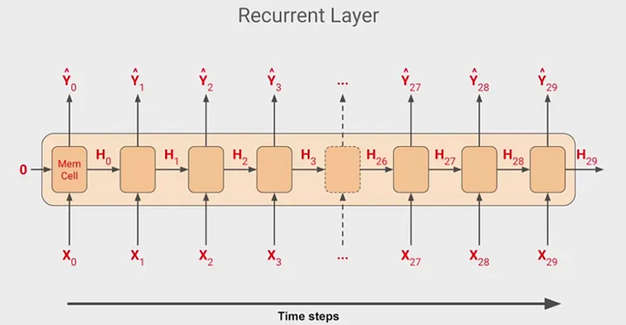
\includegraphics[width=1\textwidth]{resources/chapter-4/rnn-1.png}
\end{minipage}
\[h_t = \sigma (W_{h}x_{t} + U_h h_{t-1} + b_t) \]
\[y_t = \sigma (W_{y} h_t + b_y)\]
    \indent\textbullet\ \(h_t\): Vector lớp ẩn tại thời điểm t\\
    \indent\textbullet\ \(X_t\): vector đầu vào tại thời điểm t\\
    \indent\textbullet\ \(\widehat{Y_t}\): vector đầu ra tại thời điểm t\\
    \indent\textbullet\ \(W_h\), \(U_h\), \(W_y\): Là ma trận trọng số ngẫu nhiên\\
    \indent\textbullet\ \(b_h\), \(b_y\): là các bias\\
    \indent\textbullet\ \(\sigma_h\), \(\sigma_y\): là các hàm kích hoạt\\

Một số hàm kích hoạt phổ biến là:
\[\textbf{Sigmoid:} f(x)=\frac{1}{1+e^{-x}}, 
\ \textbf{Tanh:} f(x) = \frac{e^x - e^{-x}}{e^x + e^{-x}}\]
\[\textbf{RELU:} f(x)=\{\begin{matrix}
0 & \text{for } x<0 \\
x & \text{for } x\ge0
\end{matrix}\]
\textbf{Đầu vào}: chuỗi thời gian \(x_1\), \(x_2\), \(x_3\), ... \(x_t\), nhãn thực tế tương ứng \(y_1\), \(y_2\), \(y_3\), … \(y_t\),
\textbf{Đầu ra}: hàm mất mát (Loss Function) và cập nhật các trọng số \(W_h\), \(U_h\), \(W_y\), \(b_h\), \(b_y\)
\[\text{Loss Function} = \frac{1}{N} \sum_{i=1}^{N} (-y_i + \hat{y_i})^2\]
Lặp lại quá trình trên cho đến khi hàm mất mát giảm đủ ( không thay đổi trong một số bước lặp nhất định, không thể giảm được nữa)
% =========================================
\subsection{LSTM}
Mạng bộ nhớ dài-ngắn (Long Short Term Memory networks - LSTM), là một dạng đặc biệt của RNN, nó có khả năng học được các phụ thuộc xa. LSTM được giới thiệu bởi Hochreiter \& Schmidhuber (1997), và sau đó đã được cải tiến và phổ biến bởi rất nhiều người trong ngành. Chúng hoạt động cực kì hiệu quả trên nhiều bài toán khác nhau nên dần đã trở nên phổ biến như hiện nay.
\par
LSTM là một mạng nơ-ron tuần tự sâu trong học sâu, cho phép thông tin tồn tại lâu dài.
\par
Đây là một loại đặc biệt của Mạng Nơ-ron Tái Phát, có khả năng xử lý vấn đề vanishing gradient gặp phải bởi RNN.
    \indent\textbullet\ Output: \(c\), \(htct\), \(ht\). Ở đây, \(c\) biểu diễn trạng thái của ô (cell state) và \(h\) biểu diễn trạng thái ẩn (hidden state).
    \indent\textbullet\ Input: \(ct\)-1, \(ht\)-1\(ht\)-1, \(ht\)-1. Trong đó, \(xtxt\) là đầu vào tại trạng thái thứ \(t\) của mô hình. \(ct\)-1, \(ht\)-1\(ht\)-1, \(ht\)-1 là đầu ra từ lớp trước. \(h\) chơi vai trò tương tự như \(s\) trong RNN, trong khi \(c\) là điểm mới của LSTM.

\begin{minipage}{0.5\textwidth}
\centering
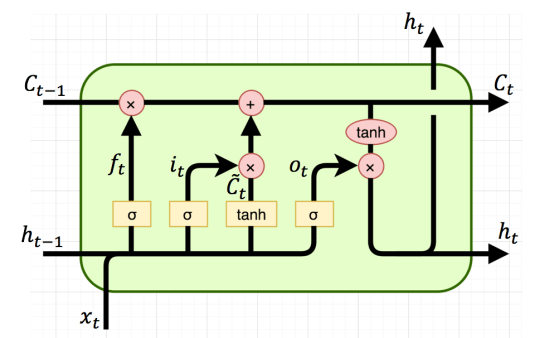
\includegraphics[width=1\textwidth]{resources/chapter-4/lstm-1.png}
\end{minipage}

Kí hiệu \(\sigma\), \(\tanh\) có nghĩa là dùng sigma, tanh và activation function
\par
\( f_t \), \( i_t \), \( o_t \) tương ứng với forget gate, input gate và output gate.\\
    \indent\textbullet\ Forget gate: \( f_t = \sigma\left(U_f \ast x_t + W_f \ast h_{t-1} + b_f\right) \)\\
    \indent\textbullet\ Input gate: \( i_t = \sigma\left(U_i \ast x_t + W_i \ast h_{t-1} + b_i\right) \)\\
    \indent\textbullet\ Output gate: \( o_t = \sigma\left(U_o \ast x_t + W_o \ast h_{t-1} + b_o\right) \)
\par
Nhận xét: \( 0 < f_t, i_t, o_t < 1 \); \( b_f, b_i, b_o \) là các hệ số bias.
\par
\( c_t = \tanh\left(U_c \ast x_t + W_c \ast h_{t-1} + b_c\right) \).
\par
\( c_t = f_t \ast c_{t-1} + i_t \ast c_t \), forget gate quyết định cần lấy bao nhiêu từ cell state trước và input gate sẽ quyết định lấy bao nhiêu từ input của state và hidden layer của layer trước.
\par
\( h_t = o_t \ast \tanh\left(c_t\right) \), output gate quyết định cần lấy bao nhiêu từ cell state để trở thành output của hidden state. Ngoài ra \( h_t \) cũng được dùng để tính output \( y_t \) cho state \( t \).


\subsection{GRU}
GRU, hoặc Gated Recurrent Unit, là một loại mạng nơ-ron hồi tiếp (RNN) được giới thiệu bởi Cho và đồng nghiệp vào năm 2014 như một phương án đơn giản hơn so với mạng LSTM (Long Short-Term Memory). Tương tự như LSTM, GRU có thể xử lý dữ liệu tuần tự như văn bản, âm thanh và dữ liệu chuỗi thời gian.
Ý tưởng cơ bản của GRU là sử dụng cơ chế cổng để lựa chọn cập nhật trạng thái ẩn của mạng tại mỗi bước thời gian. Các cơ chế cổng được sử dụng để kiểm soát luồng thông tin vào và ra khỏi mạng. GRU có hai cơ chế cổng, gọi là cổng thiết lập lại (reset gate) và cổng cập nhật (update gate).
\par
Cổng thiết lập lại xác định mức độ của trạng thái ẩn trước đó nên được quên, trong khi cổng cập nhật xác định mức độ của đầu vào mới nên được sử dụng để cập nhật trạng thái ẩn. Đầu ra của GRU được tính toán dựa trên trạng thái ẩn đã được cập nhật.LSTM là một mạng nơ-ron tuần tự sâu trong học sâu, cho phép thông tin tồn tại lâu dài.
\par
Tóm lại, mạng GRU là một loại RNN sử dụng cơ chế cổng để lựa chọn cập nhật trạng thái ẩn tại mỗi bước thời gian, cho phép chúng hiệu quả mô hình dữ liệu tuần tự. Chúng đã được chứng minh là hiệu quả trong nhiều nhiệm vụ xử lý ngôn ngữ tự nhiên, như mô hình ngôn ngữ, dịch máy và nhận dạng giọng nói.
\par
Phương trình được sử dụng để tính toán cổng thiết lập lại (\(r_t\)), cổng cập nhật (\(z_t\)), và trạng thái ẩn (\(h_t\)) của một Đơn vị Hồi tiếp Có Cổng (GRU) tại bước thời gian \(t\):

\begin{minipage}{0.5\textwidth}
\centering
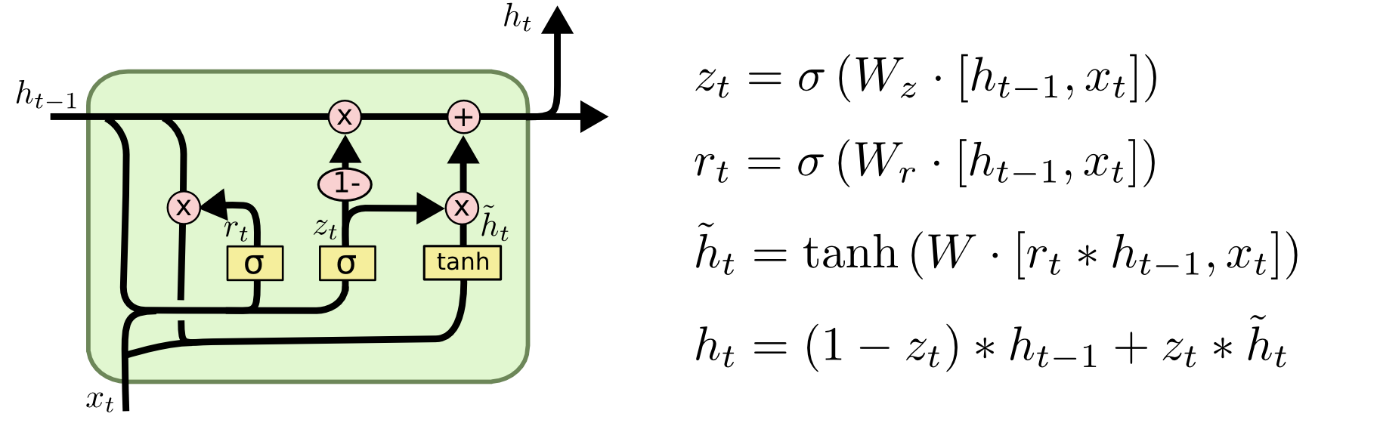
\includegraphics[width=1\textwidth]{resources/chapter-4/gru-1.png}
\end{minipage}

Trong đó:\\
    \indent\textbullet\ \(x_t\) đại diện cho đầu vào tại bước thời gian \(t\)\\
    \indent\textbullet\ \(h_{t-1}\)  là trạng thái ẩn trước đó \\
    \indent\textbullet\ \(W_r\), \(W_z\) và \(W\) là các ma trận trọng số mà mạng học được trong quá trình huấn luyện\\
    \indent\textbullet\ \(b_r\), \(b_z\) và \(b\) là các vector độ lệch\\
    \indent\textbullet\ \(\sigma\) biểu thị cho hàm sigmoid
    
% =========================================

% =========================================
\subsection{VARMA}
Vector Autoregressive Moving Average (VARMA) là mô hình thống kê dùng để mô hình hóa và dự đoán chuỗi dữ liệu có nhiều biến . VARMA là sự kết hợp giữa hai mô hình: Vector tự hồi quy (VAR) là mô hình dùng để kiểm tra các mối quan hệ giữa các biến tương tác với nhau. Trung bình trượt (MA) là mô hình thay vì sử dụng các quan sát trong quá khứ của các biến dự báo hồi quy, trung bình trượt sử dụng các lỗi dữ báo trong quá khứ. 
\par
Khi kết hợp hai mô hình lại thì mô hình VARMA được định nghĩa như sau:
\[y_{t} = c + \ \phi_{1}y_{t - 1} + \ldots + \ \phi_{p}y_{t - p} + CD_{t} + \ \theta_{1}\varepsilon_{t - 1} + \ldots + \ \theta_{q}\varepsilon_{t - p} + \ \varepsilon_{t}\]
Trong đó:\\
    \indent\textbullet\ \(y_{t}\) là vector của các biến chuỗi thời gian tại thời điểm t\\
    \indent\textbullet\ \(c\) là vector độ lệch không đổi trong mỗi phương trình\\
    \indent\textbullet\ \(\phi_{1},\ \ldots\ ,\ \phi_{p}\) là ma trận tham số của AR với i = 1, …, p\\
    \indent\textbullet\ \(C\) là ma trận hệ số của các biến hồi quy có khả năng xác định\\
    \indent\textbullet\ \(D_{t}\) là vector chứa các biến hồi quy xác định thích hợp như biến không đổi, xu hướng hoặc mùa vụ\\
    \indent\textbullet\ \(\theta_{1},\ \ldots\ ,\ \theta_{p}\) là ma trận tham số của MA với j = 1, … , q\\
    \indent\textbullet\ \(\varepsilon_{t}\) là vector lỗi ngẫu nhiêu tại thời điểm t\\

% =========================================
% =========================================
\subsection{Kalman Filter}
\subsubsection{Định nghĩa}
Kalman Filter là một thuật toán tổng quát được sử dụng để ước lượng các tham số hệ thống. Nó có thể sử dụng các đo lường không chính xác hoặc nhiễu để ước lượng trạng thái của biến đó hoặc một biến không quan sát được khác với độ chính xác cao hơn.
\par
Sức mạnh thực sự của Kalman Filter không phải là làm mịn các đo lường. Mà đó là khả năng ước lượng các tham số hệ thống mà không thể được đo lường hoặc quan sát với độ chính xác. Các ước lượng có độ chính xác cải thiện trong các hệ thống hoạt động thời gian thực, cho phép hệ thống kiểm soát mạnh mẽ hơn và do đó có nhiều khả năng hơn.

\subsubsection{Công thức}

\begin{minipage}{0.45\textwidth}
\centering
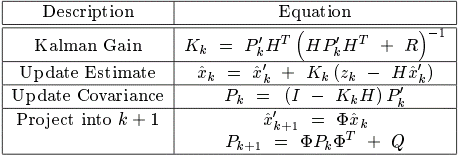
\includegraphics[width=1\textwidth]{resources/chapter-4/kalman-fillter-1.png}
\end{minipage}
\\ \\
Trong đó:\\
    \indent\textbullet\ K là Kalman Gain\\
    \indent\textbullet\ P là Ma trận hiệp phương sai\\
    \indent\textbullet\ H là ma trận quan sát \\
    \indent\textbullet\ \(H^T\) là mà trận chuyên vị của H\\
    \indent\textbullet\ \(Z_k\) là giá trị đo được (tại thời điểm k)\\
    \indent\textbullet\ \(X_k\) là giá trị dự đoán (tại thời điểm k)

\subsubsection{Cách thuật toán hoạt động}
    \indent\textbullet\ Bước 1: Khởi tạo giá trị ban đầu của X và P bằng với giá trị đầu tiên của bộ dữ liệu\\
    \indent\textbullet\ Bước 2: Sau đó sẽ tiến hành dự đoán \(X_{k^-}\) và \(P_{k^-}\) (Giá trị trước khi đo đạc)\\
    \indent\textbullet\ Bước 3: Tính toán lại Kalman Gain\\
    \indent\textbullet\ Bước 4: Sau khi đo lường được giá trị \(Z_k\) thì sẽ tính toán lại \(X_k\)(Giá trị dự đoán)\\
    \indent\textbullet\ Bước 5: Sau đó sẽ tính toán lại P và lặp lại từ bước 2\\

\begin{minipage}{0.45\textwidth}
\centering
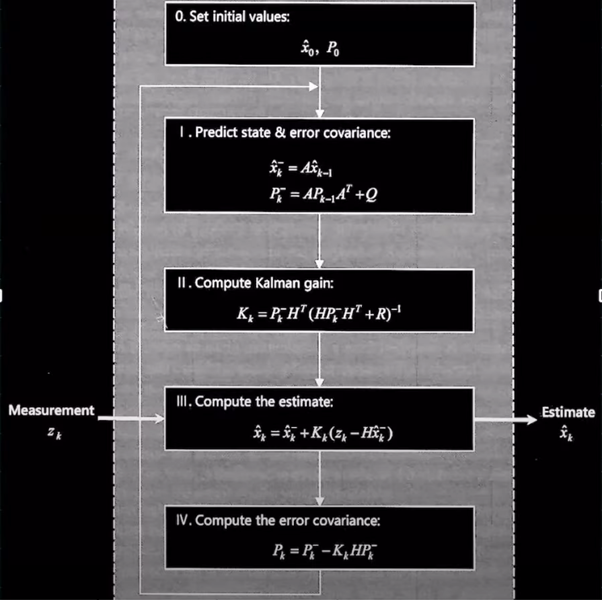
\includegraphics[width=1\textwidth]{resources/chapter-4/kalman-fillter-2.png}
\end{minipage}
\\ \\

% =========================================
\subsection{Meta-learning}
Meta-learning là một phương pháp trong học máy nhằm huấn luyện các mô hình để học một cách hiệu quả các nhiệm vụ mới với lượng dữ liệu hạn chế. Một trong những thuật toán nổi tiếng nhất trong meta-learning là Model-Agnostic Meta-Learning (MAML).
\par
\textbf{Model-Agnostic Meta-Learning (MAML)}
\par
Mục tiêu: MAML nhằm tìm một khởi tạo tốt cho các tham số của mô hình, giúp mô hình có thể được tinh chỉnh nhanh chóng trên một nhiệm vụ mới chỉ với một vài bước cập nhật gradient.
\par
\textbf{Khái niệm chính}
\par
    \indent\textbullet\ 1.	Phân phối nhiệm vụ (p(T)p(T)): Một phân phối trên các nhiệm vụ mà mô hình cần thích nghi.\\
    \indent\textbullet\ 2.	Mô hình cơ bản (\(f_\theta f_\theta\)): Mô hình được tham số hóa bởi \(\theta \theta\).\\
    \indent\textbullet\ 3.	Bộ dữ liệu hỗ trợ (Support Set): Bộ dữ liệu nhỏ từ đó mô hình học nhiệm vụ.\\
    \indent\textbullet\ 4.	Bộ dữ liệu truy vấn (Query Set): Bộ dữ liệu được dùng để đánh giá mô hình sau khi nó đã thích nghi với nhiệm vụ.\\
\par
\textbf{Các bước của thuật toán MAML}
\par
    \indent\textbullet\ 1.	Khởi tạo tham số mô hình: Bắt đầu với các tham số khởi tạo \(\theta \theta\).\\
    \indent\textbullet\ 2.	Lấy mẫu một loạt các nhiệm vụ: Lấy mẫu một loạt các nhiệm vụ {Ti}{Ti} từ phân phối nhiệm vụ p(T)p(T)\\
    \indent\textbullet\ 3. Đối với mỗi nhiệm vụ \(T_i\)\\
    	Lấy mẫu bộ dữ liệu hỗ trợ \(D_{T_i}^{\mathrm{train\ }}\) và bộ dữ liệu truy vấn \(D_{T_i}^{\mathrm{test\ }}\).\\ \\
     	Tính gradient của hàm mất mát trên bộ dữ liệu hỗ trợ với tham số \(\theta\):\\
            \[\nabla_\theta\mathcal{L}_{T_i}\left(f_\theta\right)\] \\
            Cập nhật các tham số sử dụng gradient:\\
            \[\theta_i^\prime=\theta-\alpha\nabla_\theta\mathcal{L}_{T_i}\left(f_\theta\right)\] \\
        \indent\textbullet\ 4. Cập nhật Meta\\
            Tính hàm mất mát trên bộ dữ liệu truy vấn sử dụng tham số đã cập nhật \(\theta_i^\prime\) \\ 
            \[\mathcal{L}_{T_i}\left(f_{\theta_i^\prime}\right)\]\\
            Tính gradient của hàm mất mát trên bộ dữ liệu truy vấn đối với các tham số khởi tạo \(\theta\) \\
            \[\nabla_\theta\mathcal{L}_{T_i}\left(f_{\theta_i^\prime}\right)\] \\
            Cập nhật các tham số khởi tạo \(\theta\) bằng cách trung bình các gradient qua loạt nhiệm vụ: \\
            \[\theta \gets \theta - \beta \sum_{i} \, \nabla_{\theta} \mathcal{L}_{T_{i}} \left( f_{\theta_{i}^{\prime}} \right)\]
            , với \(\beta\) là tốc độ học của meta.

% =========================================
\subsection{NBeats}
\begin{minipage}{0.45\textwidth}
\centering
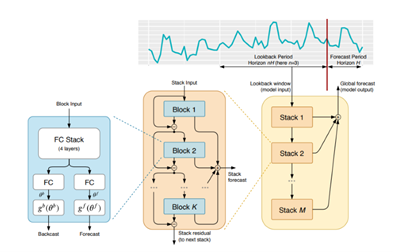
\includegraphics[width=1\textwidth]{resources/chapter-4/nbeats-1.png}
\end{minipage}
\\
\({h}_{\ell,1} = FC_{\ell,1}({x}_{\ell}), \quad {h}_{\ell,2} = FC_{\ell,2}({h}_{\ell,1}), \quad {h}_{\ell,3} = FC_{\ell,3}({h}_{\ell,2}), \quad {h}_{\ell,4} = FC_{\ell,4}({h}_{\ell,3}).\) \\
\(\theta^b_{\ell} = LINEAR_{\ell}^{b}({h}_{\ell,4}), \quad \theta^f_{\ell} = LINEAR_{\ell}^{f}({h}_{\ell,4}).\) \\

\[\widehat{\vec{y}}_{\ell} = \sum_{i=1}^{\dim(\theta^f_{\ell})} \theta^f_{\ell,i} \vec{v}^f_{i}, \quad  \widehat{\vec{x}}_{\ell} = \sum_{i=1}^{\dim(\theta^b_{\ell})} \theta^b_{\ell,i} \vec{v}^b_{i}.
\]
Mô tả cấu trúc mô hình: \\
\\
\textbf{Khối Đầu vào (Time series input)}: của mô hình là một chuỗi thời gian \(Y_{t-n+1:t}\) chứa các đặc điểm của quá khứ.\\
\textbf{Ngăn xếp khối đầu vào (Stack Input)}: cấu trúc này bao gồm các khối được xếp chống lên nhau. Mỗi khối thực hiện 2 nhiệm vụ chính là dự đoán lại quá khư (backcast) và dự báo tương lai(forecast)\\
\textbf{Broadcast}: mỗi khối cố  gắng tại tạo lại đầu vào (phần quá khứ) để dảm phần dư trước khi chuyển trang khối tiếp theo\\
\textbf{Forecast}: Mỗi khi đưa ra dự báo cho tương lai và các dự báo này được tổng hợp lại để tạo ra dự báo cuối cùng\\
\\
\textbf{Fully Connected Layers}: Mỗi khối báo gồm nhiều lớp fully-connected. Các lớp này sử dụng các hàm kích hoạt để học các bieuer diễn phi tuyến của dữ liệu\\
\textbf{Residual Connections(kết nối dư)}: sau mỗi khối, phần dư giữa đầu vào và backcast được tính toán và sử dụng làm đầu vào cho khối tiếp theo\\
\textbf{Global Forcecast}: Dự báo cuối cùng được tạo ra bằng cách tổng hợp các dự báo từ tát cả các khối. Các dự báo này được kết hợp lại để tạo ra dự báo cuối cùng cho chuỗi thời gian tương lai.\\

% =========================================
\subsection{N-HiTS}
\begin{minipage}{0.45\textwidth}
\centering
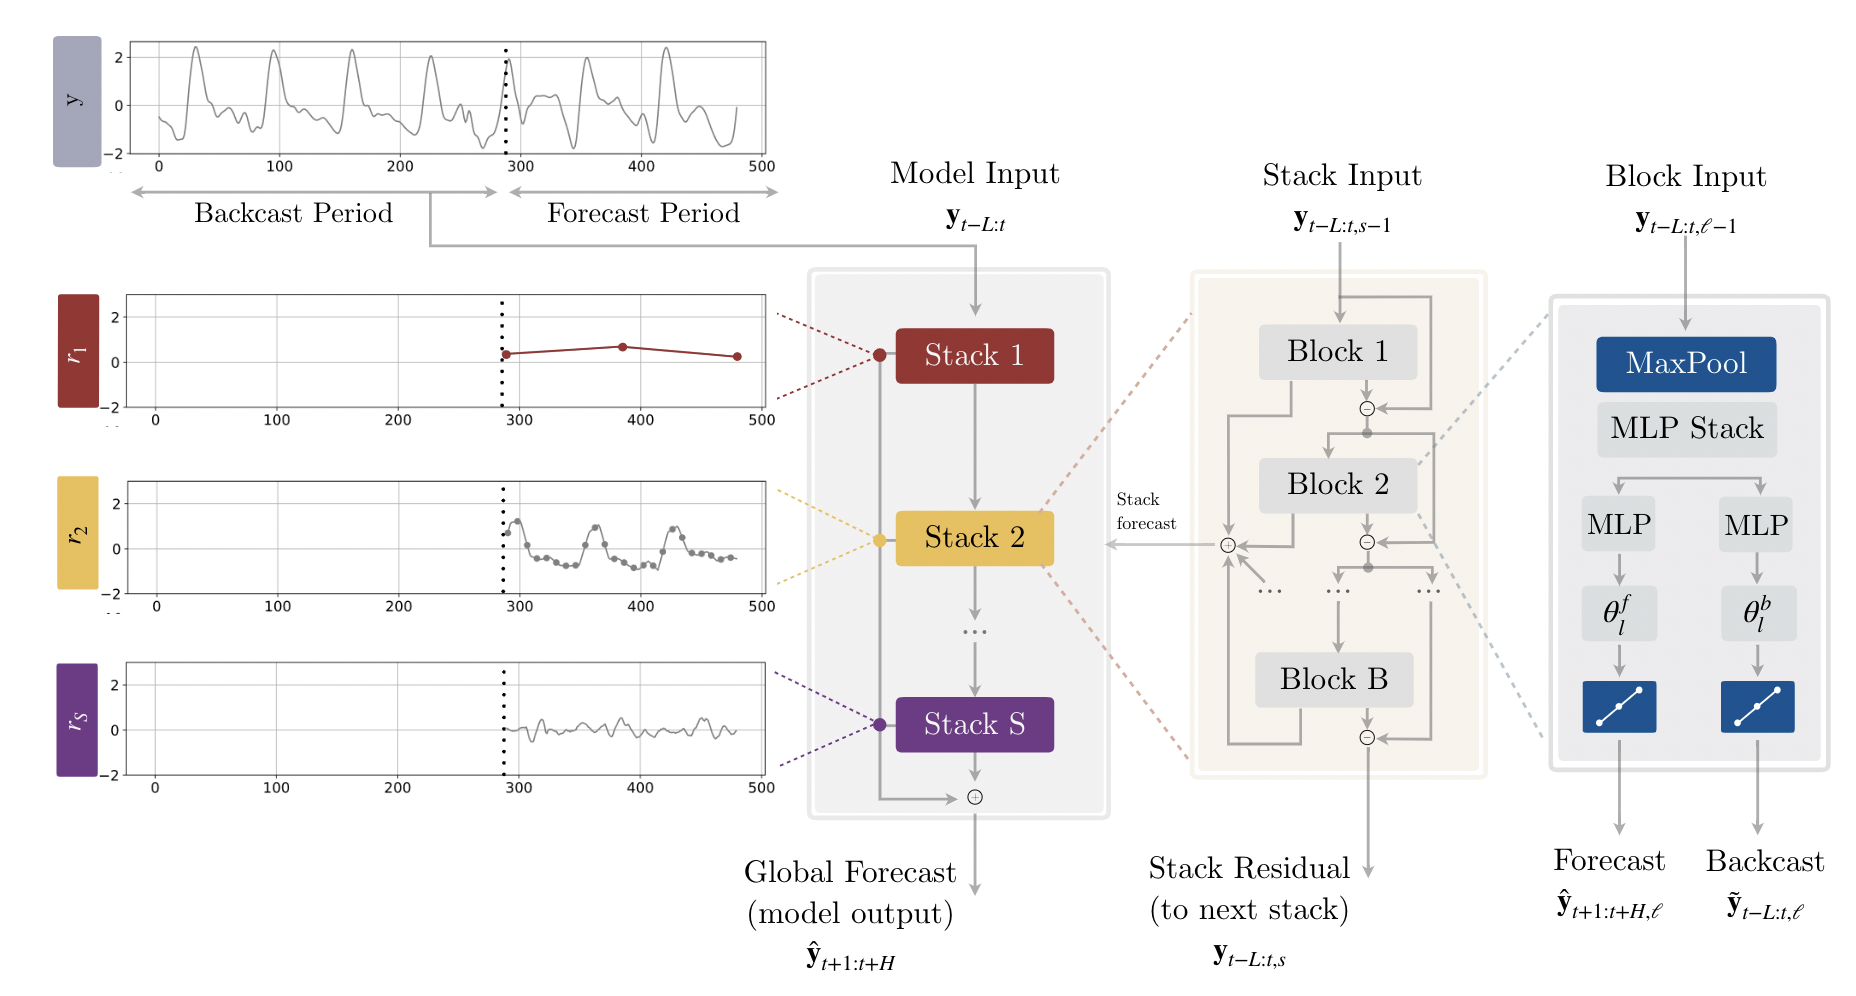
\includegraphics[width=1\textwidth]{resources/chapter-4/nhits-1.png}
\end{minipage}

N-HiTS là một phương pháp dự báo chuỗi thời gian, mở rộng từ phương pháp Neural Basis Expansion Analysis (N-BEATS). N-HiTS cải thiện độ chính xác và hiệu quả tính toán, đặc biệt trong dự báo dài hạn, thông qua việc sử dụng lấy mẫu đa tỷ lệ và tổng hợp đa tỷ lệ.

\textbf{Nguyên lý hoạt động:}
Giống như N-BEATS, N-HiTS thực hiện các phép chiếu phi tuyến cục bộ lên các hàm cơ sở qua nhiều khối, mỗi khối bao gồm một multilayer perceptron (MLP) học cách tạo ra các hệ số cho đầu ra backcast và forecast. Các khối được nhóm thành các stack, mỗi stack học một đặc điểm khác nhau của dữ liệu. Đầu vào của toàn bộ mạng là chuỗi tín hiệu \(y_{t-L:t}\) từ \(L\) độ trễ.

\textbf{Lấy mẫu tín hiệu đa tỷ lệ:}
Tại đầu vào của mỗi khối \(\ell\), một lớp MaxPool với kích thước kernel \(k_{\ell}\) được sử dụng để phân tích các thành phần tín hiệu ở một tỷ lệ cụ thể. Kích thước \(k_{\ell}\) lớn hơn cắt bớt các thành phần tần số cao, giúp khối tập trung vào phân tích các nội dung quy mô lớn. Điều này giúp giảm số lượng tham số cần học, giảm thiểu overfitting và duy trì trường tiếp nhận ban đầu.
\[\mathbf{y}^{(p)}_{t-L:t, \ell} = \mathbf{MaxPool}\left(\mathbf{y}_{t-L:t, \ell},\; k_{\ell}\right)\]

\textbf{Hồi quy phi tuyến:}
Sau khi lấy mẫu, khối thực hiện hồi quy phi tuyến để tạo ra các hệ số MLP tiến và lùi. Các hệ số này được sử dụng để tổng hợp đầu ra backcast và forecast của khối. Quá trình này giúp tạo ra dự báo chính xác hơn bằng cách sử dụng các phép chiếu phi tuyến.
\begin{align*}
\begin{split}
    {h}_{\ell} = \mathbf{MLP}_{\ell}\left(\mathbf{y}^{(p)}_{t-L:t,\ell}\right)\\
    \theta^{f}_{\ell} = \textbf{LINEAR}^{f}\left(\mathbf{h}_{\ell}\right)\\
    \theta^{b}_{\ell} = \textbf{LINEAR}^{b}\left(\mathbf{h}_{\ell}\right)
\end{split}
\end{align*}

\textbf{Nội suy phân cấp (Hierarchical Interpolation):}
Để giải quyết vấn đề tăng nhanh yêu cầu tính toán khi chân trời dự báo tăng, N-HiTS sử dụng nội suy thời gian. Các hệ số nội suy được xác định theo tỷ lệ biểu đạt (expressiveness ratio) \(r_{\ell}\) điều chỉnh số lượng tham số trên mỗi đơn vị thời gian đầu ra, $|\theta^{f}_{\ell}|= \lceil r_{\ell} \, H \rceil$. Để khôi phục lại tốc độ lấy mẫu ban đầu và dự báo tất cả $H$ điểm trong tầm nhìn, chúng ta sử dụng nội suy thời gian thông qua hàm nội suy $g$:
\begin{align*}
\begin{split}
    \hat{y}_{\tau,\ell}   = g(\tau, \theta^{f}_{\ell}), \quad \forall \tau \in \{t+1,\dots,t+H\}, \\
    \tilde{y}_{\tau,\ell} = g(\tau, \theta^{b}_{\ell}), \quad \forall \tau \in \{t-L,\dots,t\}. 
\end{split}
\end{align*}